\documentclass[hyperref={pdfpagelabels=false},aspectratio=34,14pt]{beamer}
\usepackage{lmodern} %TODO: descobrir o que mudou as fontes dos slides (comparar com os primeiros)
\usepackage[utf8]{inputenc}
\usepackage[T1]{fontenc}
\usefonttheme[onlymath]{serif}
\usepackage[brazil]{babel}
\usepackage[outputdir=..]{minted}
\usepackage{xcolor}
\usepackage{soul} % strikethrough
\usepackage{advdate}
\usepackage{graphicx}
\usepackage[ampersand]{easylist}
\usepackage{multirow}
\usepackage{tikz}
\usetikzlibrary{shapes,arrows,positioning}
\usetikzlibrary{circuits.logic.US}
\usetikzlibrary{matrix,calc}
\usepackage{karnaugh-map}

\usepackage{pgfpages}
\setbeamertemplate{note page}{\pagecolor{yellow!5}\insertnote}\usepackage{palatino}
\newcommand{\yes}{edge node [above] {yes}}
\newcommand{\no}{edge  node [left]  {no}}
\newcommand{\textttb}[1]{\textcolor{blue}{\ttfamily #1}}

% \setmathfont{Latin Modern Math}[version=lm]

\graphicspath{{../figs/}}

\definecolor{bgc}{rgb}{0.95,0.9,0.95}
\definecolor{links}{HTML}{2A7F7F}
\hypersetup{colorlinks,linkcolor=,urlcolor=links}

\newminted{verilog}{fontsize=\scriptsize, 
		   linenos,
		   numbersep=8pt,
           bgcolor=bgc,
           tabsize=4,
		   framesep=3mm} 
%		   frame=lines,

\newcommand{\verilog}[1]{\verilogf{#1}{\footnotesize}

\newcommand{\verilogf}[2]{\inputminted[fontsize=#2, 
		   linenos,
		   tabsize=2,
		   numbersep=4pt,
           bgcolor=bgc,
		   framesep=3mm]{verilog}{../codes/#1.v}
}

\newminted{nasm}{fontsize=\scriptsize, 
		   linenos,
		   numbersep=8pt,
           bgcolor=bgc,
		   framesep=3mm} 

% \author[shortname]{\scriptsize Prof. Edilson Kato \and Prof. Maurício Figueiredo \and Prof. Ricardo Menotti\newline
% \href{mailto:kato@ufscar.br}{kato@ufscar.br} \and    \href{mailto:mauricio@ufscar.br}{mauricio@ufscar.br} \and
% \href{mailto:menotti@ufscar.br}{menotti@ufscar.br}}

\newcommand{\newauthor}[2]{
  \parbox{0.40\textwidth}{
    \texorpdfstring
      {
        \centering
        \footnotesize #1 \newline
        {\scriptsize{\urlstyle{same}\href{mailto:#2}{#2}\urlstyle{tt}}}
      }
      {#1} \newline
  }
}

\author{
%   \newauthor{Prof. Edilson Kato}{kato@ufscar.br}
% \and
  \newauthor{Prof. Ricardo Menotti}{menotti@ufscar.br}
\and 
  \newauthor{Prof. Maurício Figueiredo}{mauricio@ufscar.br}
% \and
%   \newauthor{Prof. Roberto Inoue}{rsinoue@ufscar.br}
}

\institute{\href{http://www.dc.ufscar.br/}{Departamento de Computação} \\
           \href{http://www.ufscar.br/}{Universidade Federal de São Carlos}} 
\titlegraphic{
  \makebox[.85\paperwidth]{
    
\includegraphics[height=1cm]{figs/LogoDC} 
    \hfill 
    
\includegraphics[height=1cm]{figs/LogoUfscar}}}
\date{Atualizado em: \today} 
% \date{\DayAfter[+1]} % +/-

%\logo{
\includegraphics[height=1cm]{figs/LogoUfscar}
\includegraphics[height=1cm]{figs/LogoDC}}

\title{Lógica Digital (1001351)}

\AtBeginSubsection[]
{
  \begin{frame}<beamer>{Roteiro}
    \tableofcontents[currentsection,currentsubsection]
  \end{frame}
}

\addtobeamertemplate{navigation symbols}{}{%
    \usebeamerfont{footline}%
    \usebeamercolor[fg]{footline}%
    \hspace{1em}%
    \raisebox{1.2pt}[0pt][0pt]{\insertframenumber/\inserttotalframenumber}
}


\title{Introdução à Computação Reconfigurável}

\subtitle{Laboratório de Organização e Arquitetura de Computadores I}

\begin{document}

\begin{frame}
	\titlepage
\end{frame} 

\begin{frame}{Conteúdo}
	\tableofcontents
\end{frame}

\section{Introdução} %%%%%%%%%%%%%%%%%%%%%%%%%%%%%%%%%%%%%%%%%%%%%%%%%%%%%%%%%%%%%%%%%%%%%%

\begin{frame}{Métodos de computação \cite{menotti2010.phd}} 
	\center	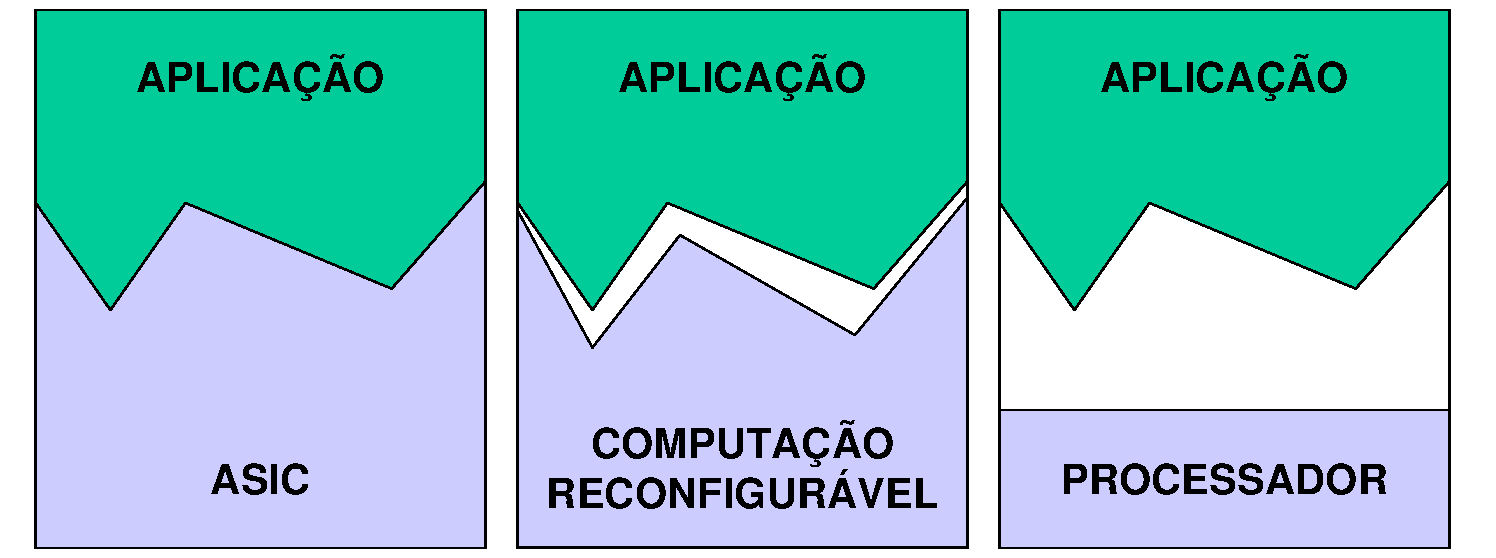
\includegraphics[width=\textwidth]{gap}
\end{frame}

\begin{frame}{Mercado de lógica digital \cite{hamblen}} 
	\center	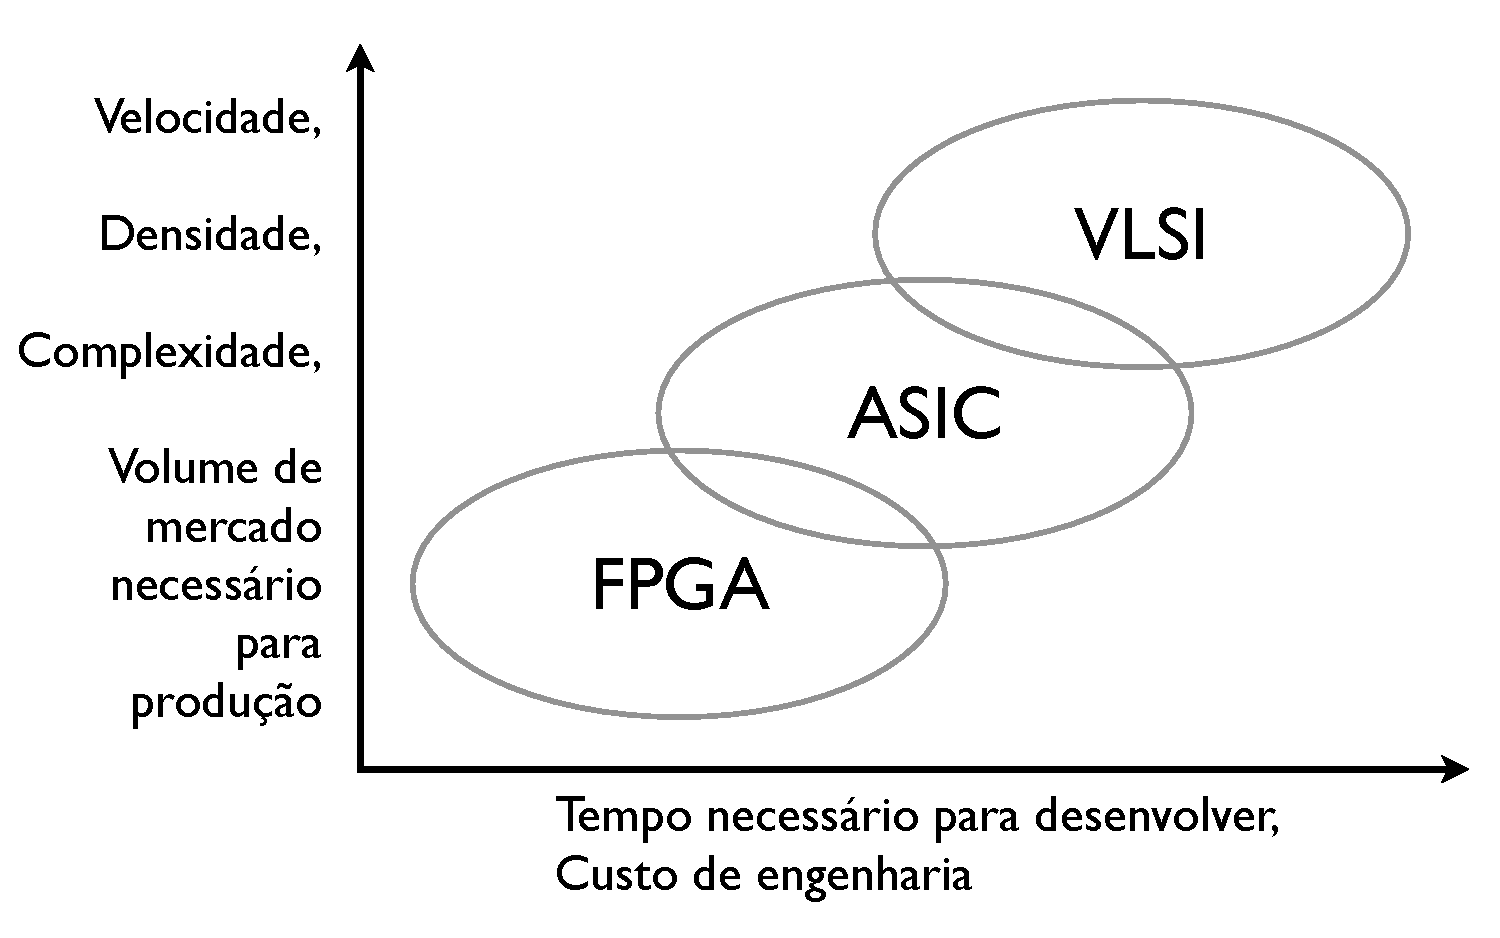
\includegraphics[height=.75\textheight]{market}
\end{frame}

\begin{frame}{Relação entre flexibilidade e desempenho \cite{bobda}} 
	\center	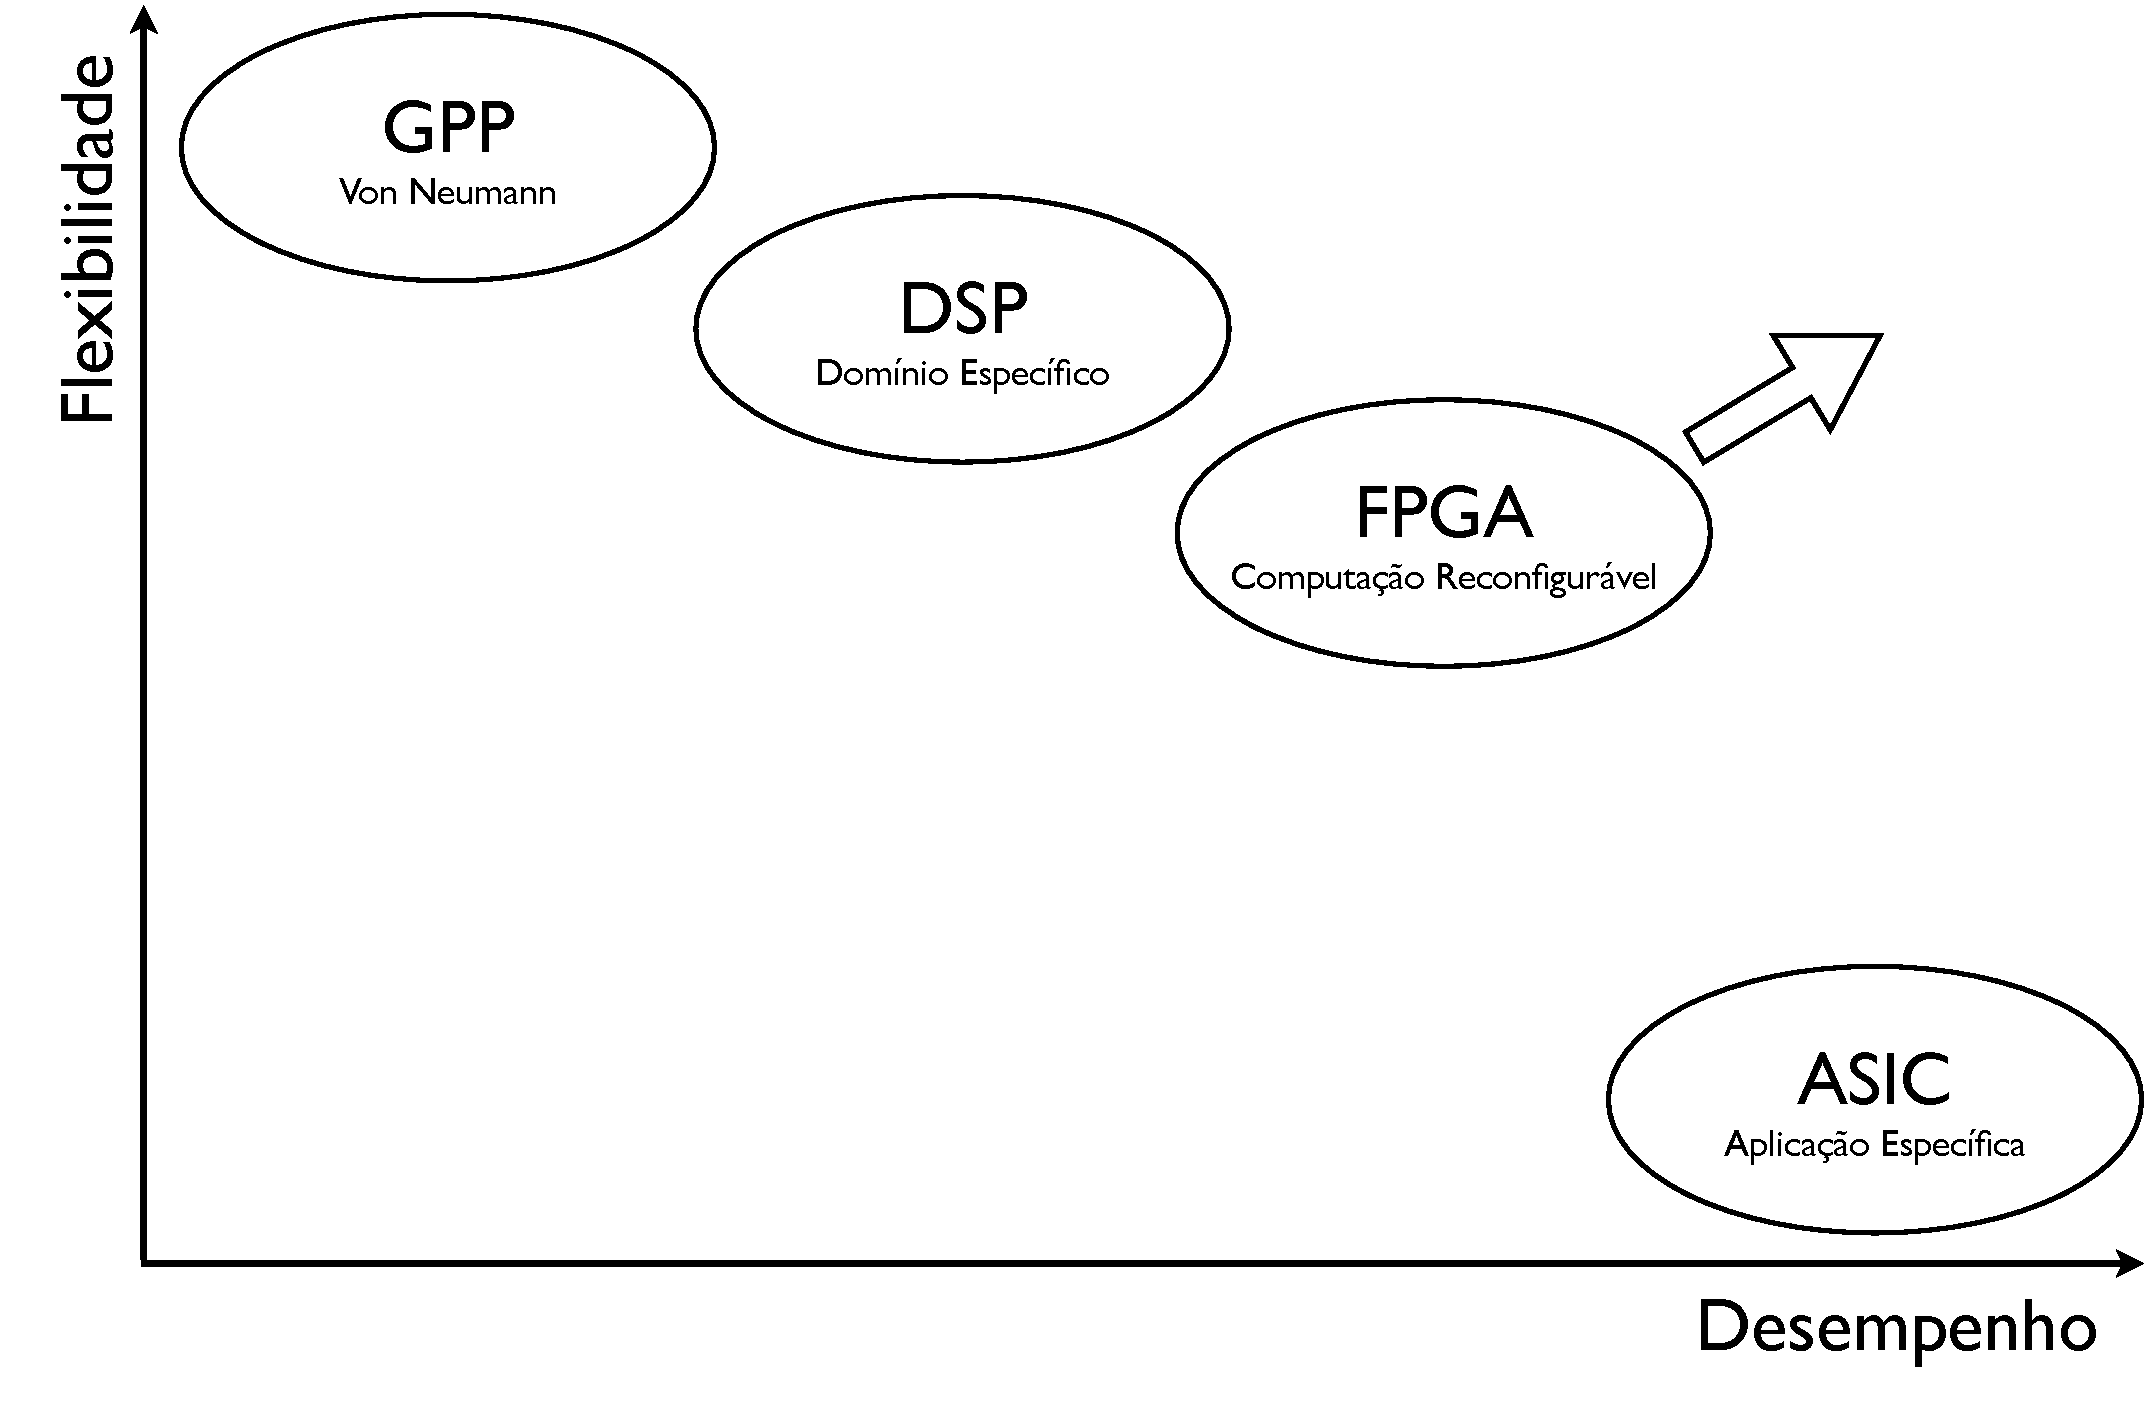
\includegraphics[height=.75\textheight]{FlexDesemp}
\end{frame}

\section{FPGAs} %%%%%%%%%%%%%%%%%%%%%%%%%%%%%%%%%%%%%%%%%%%%%%%%%%%%%%%%%%%%%%%%%%%%%%

\begin{frame}{Estrutura básica de um FPGA} 
	\center	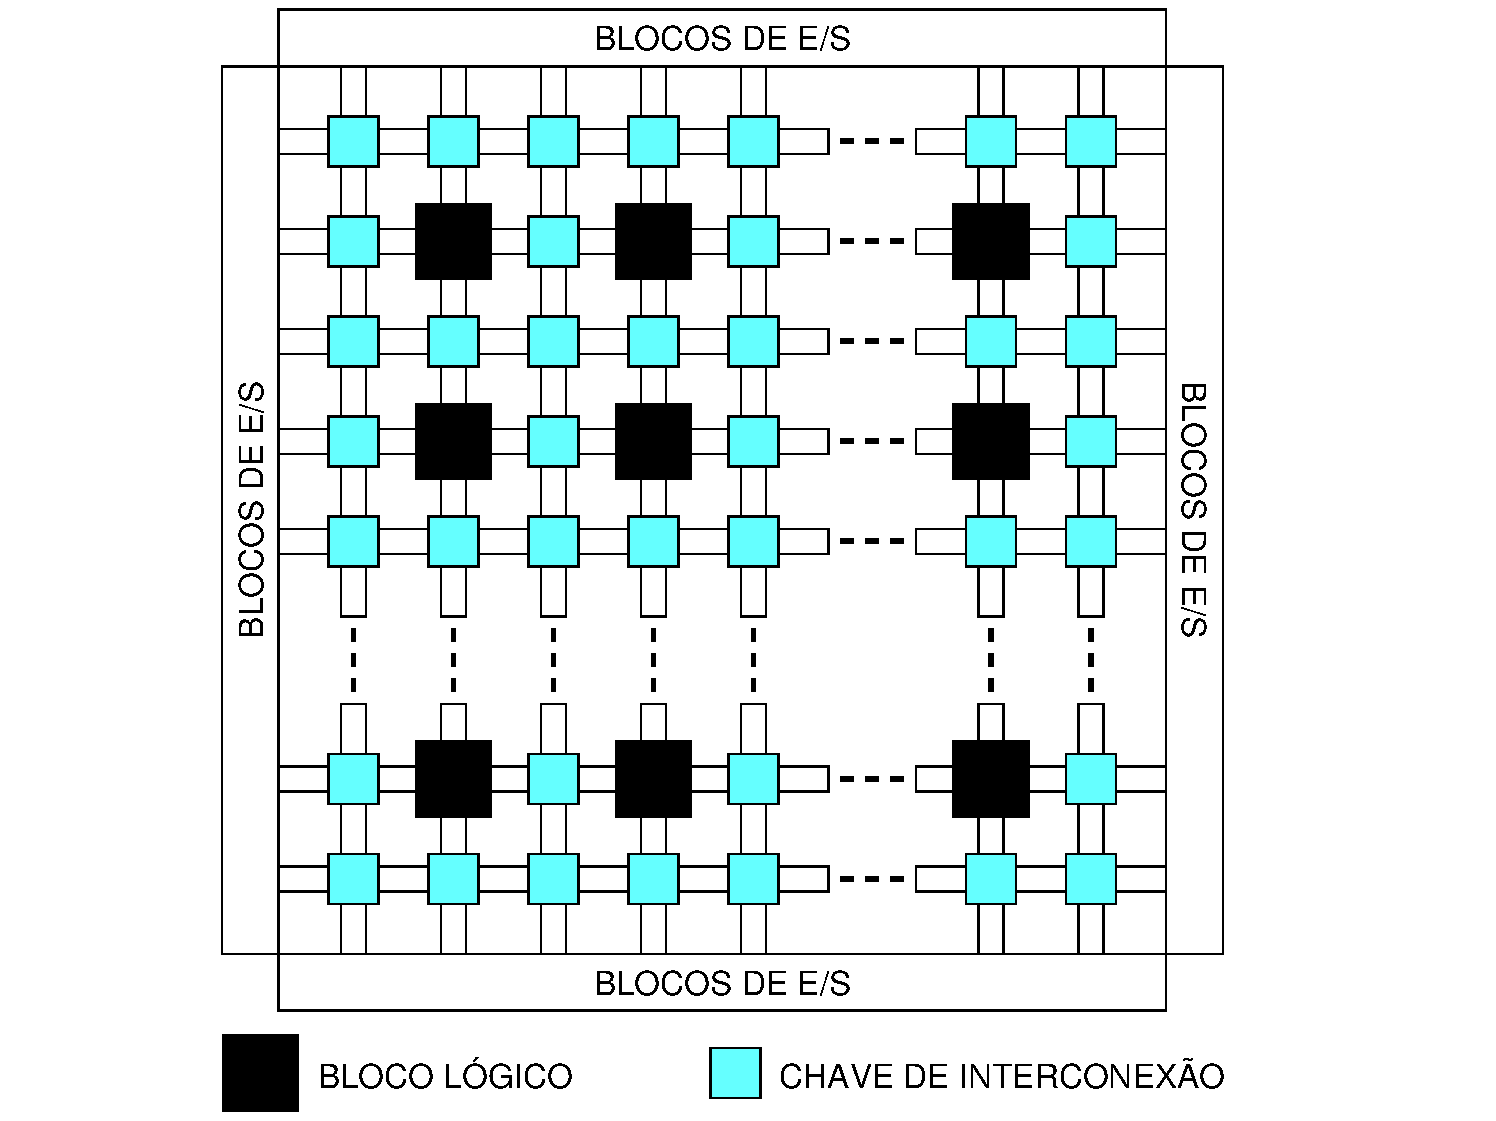
\includegraphics[height=.75\textheight]{fpgafig}
\end{frame}

\begin{frame}{Uso de LUTs para implementação de funções lógicas} 
	\center	
    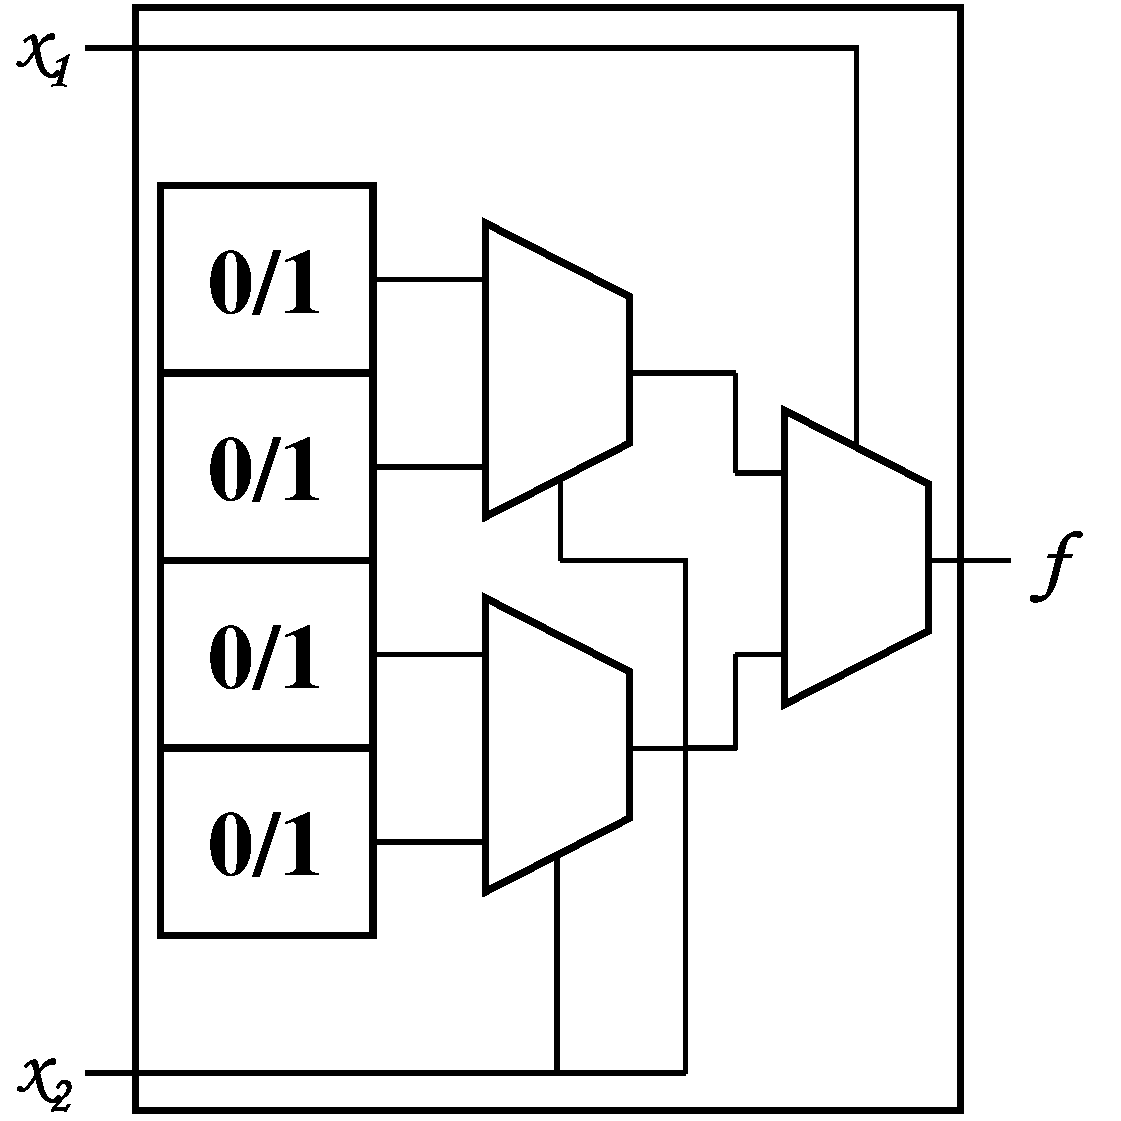
\includegraphics[width=.3\textwidth]{lut01}
	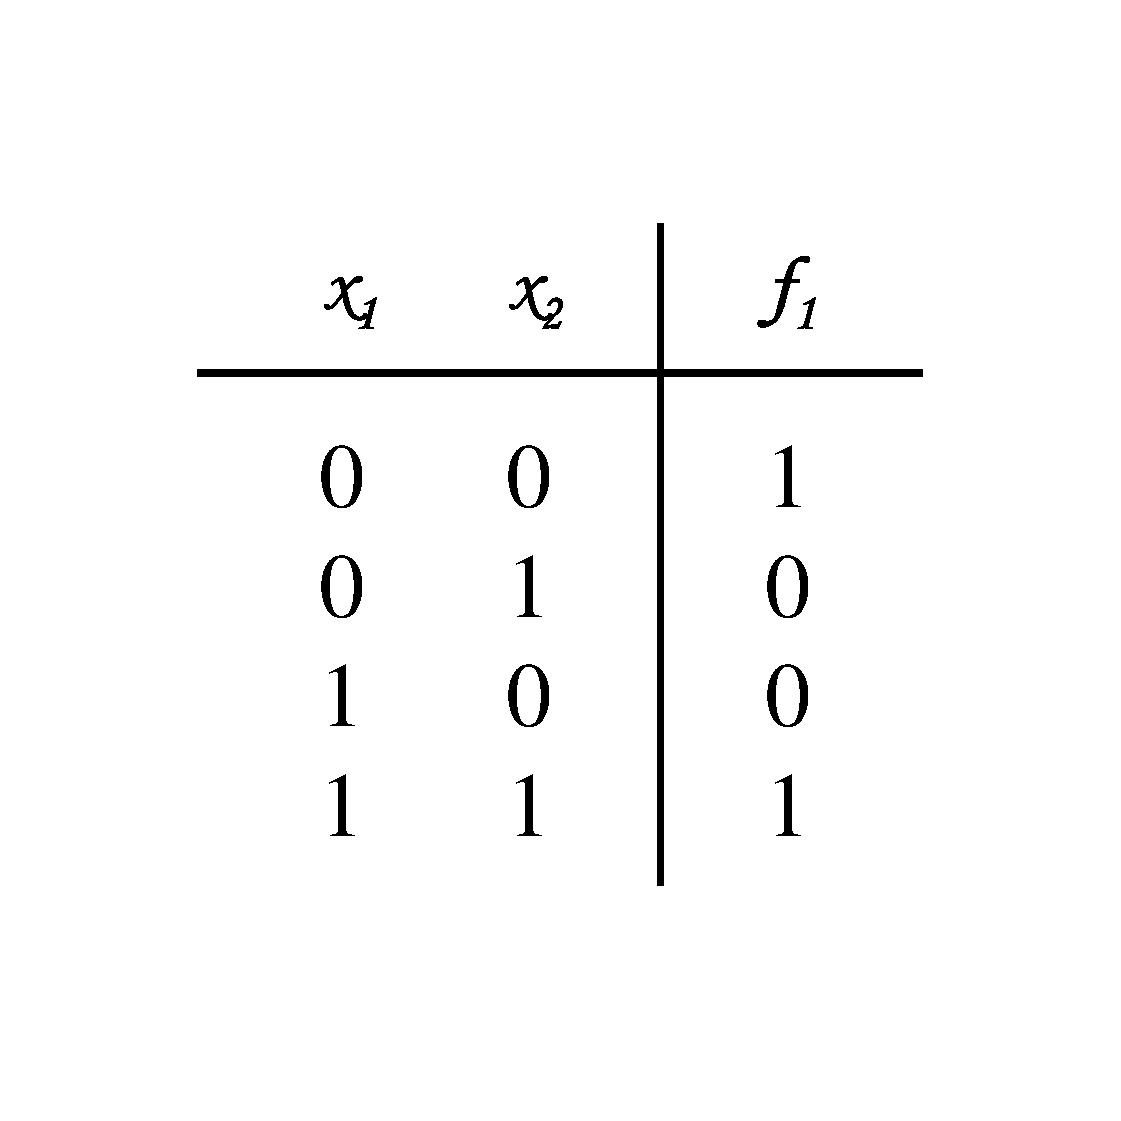
\includegraphics[width=.35\textwidth]{func}
    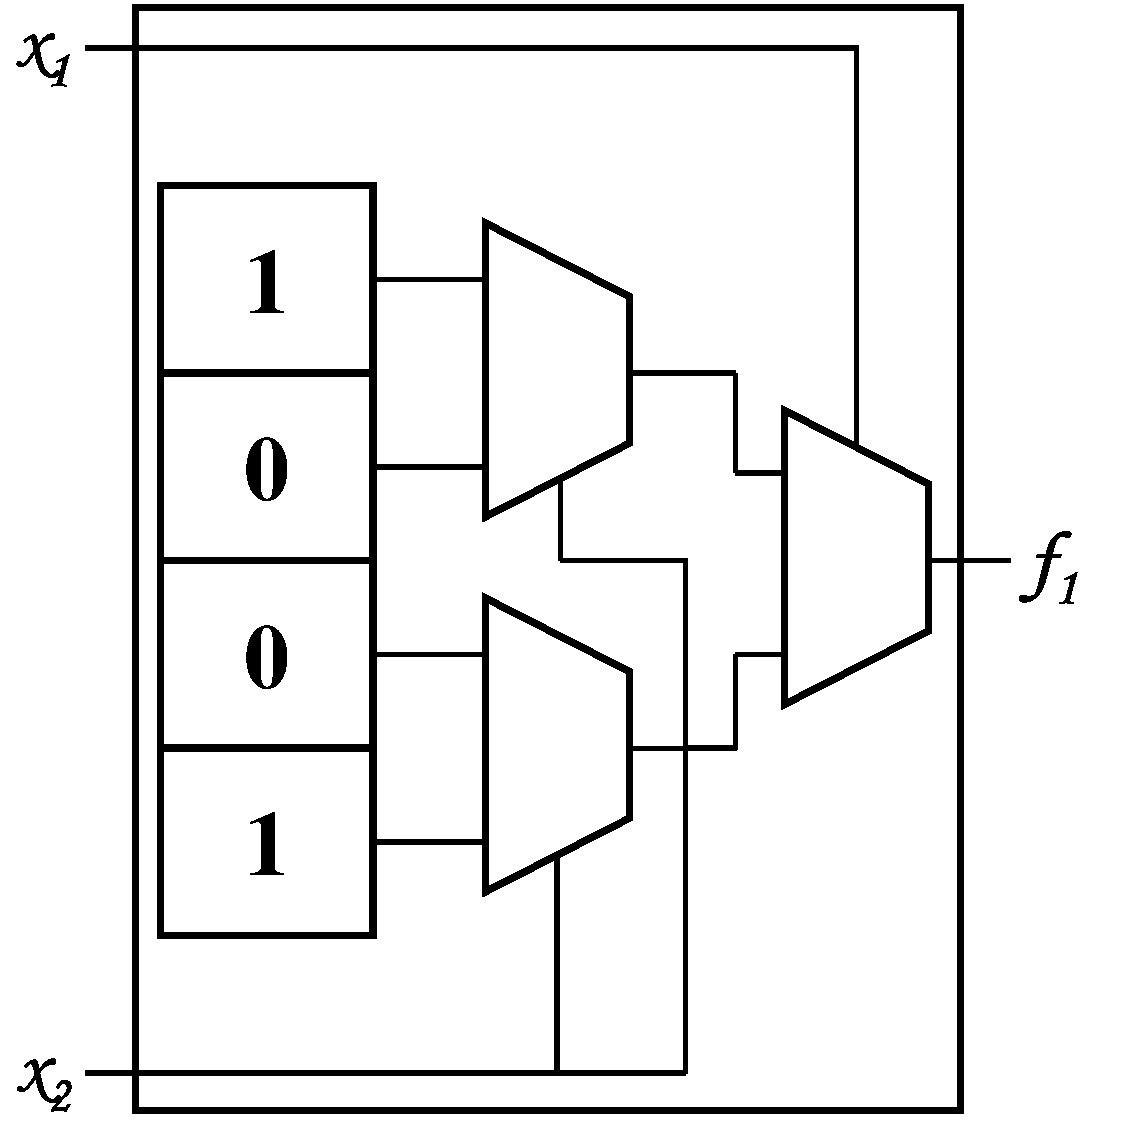
\includegraphics[width=.3\textwidth]{lut}
\end{frame}

\begin{frame}{Circuito de uma LUT de três entradas} 
	\center	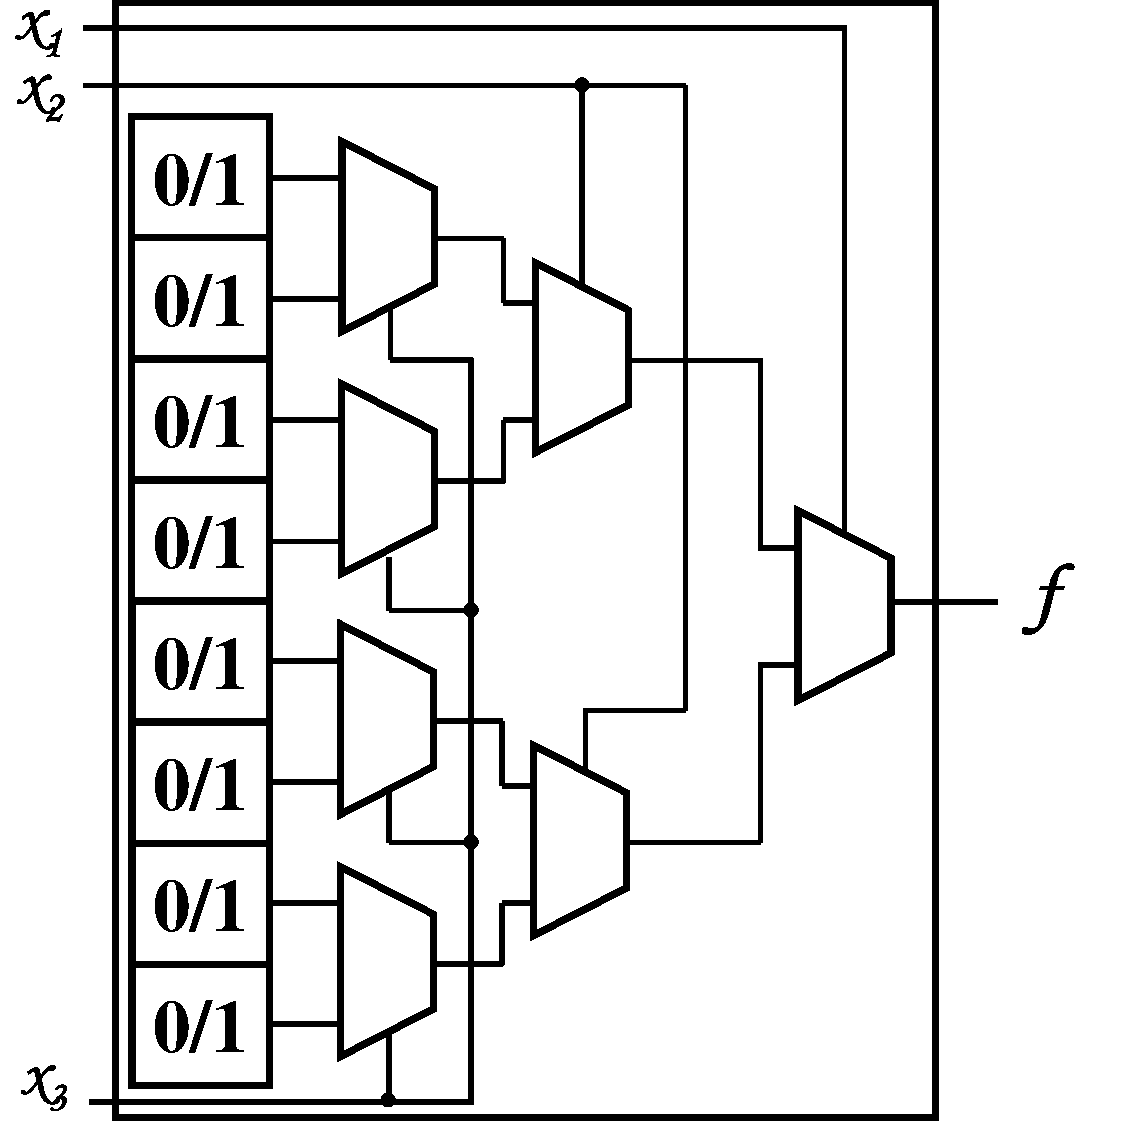
\includegraphics[width=.5\textwidth]{lut3}
\end{frame}

\begin{frame}{Elementos Lógicos}
	\center	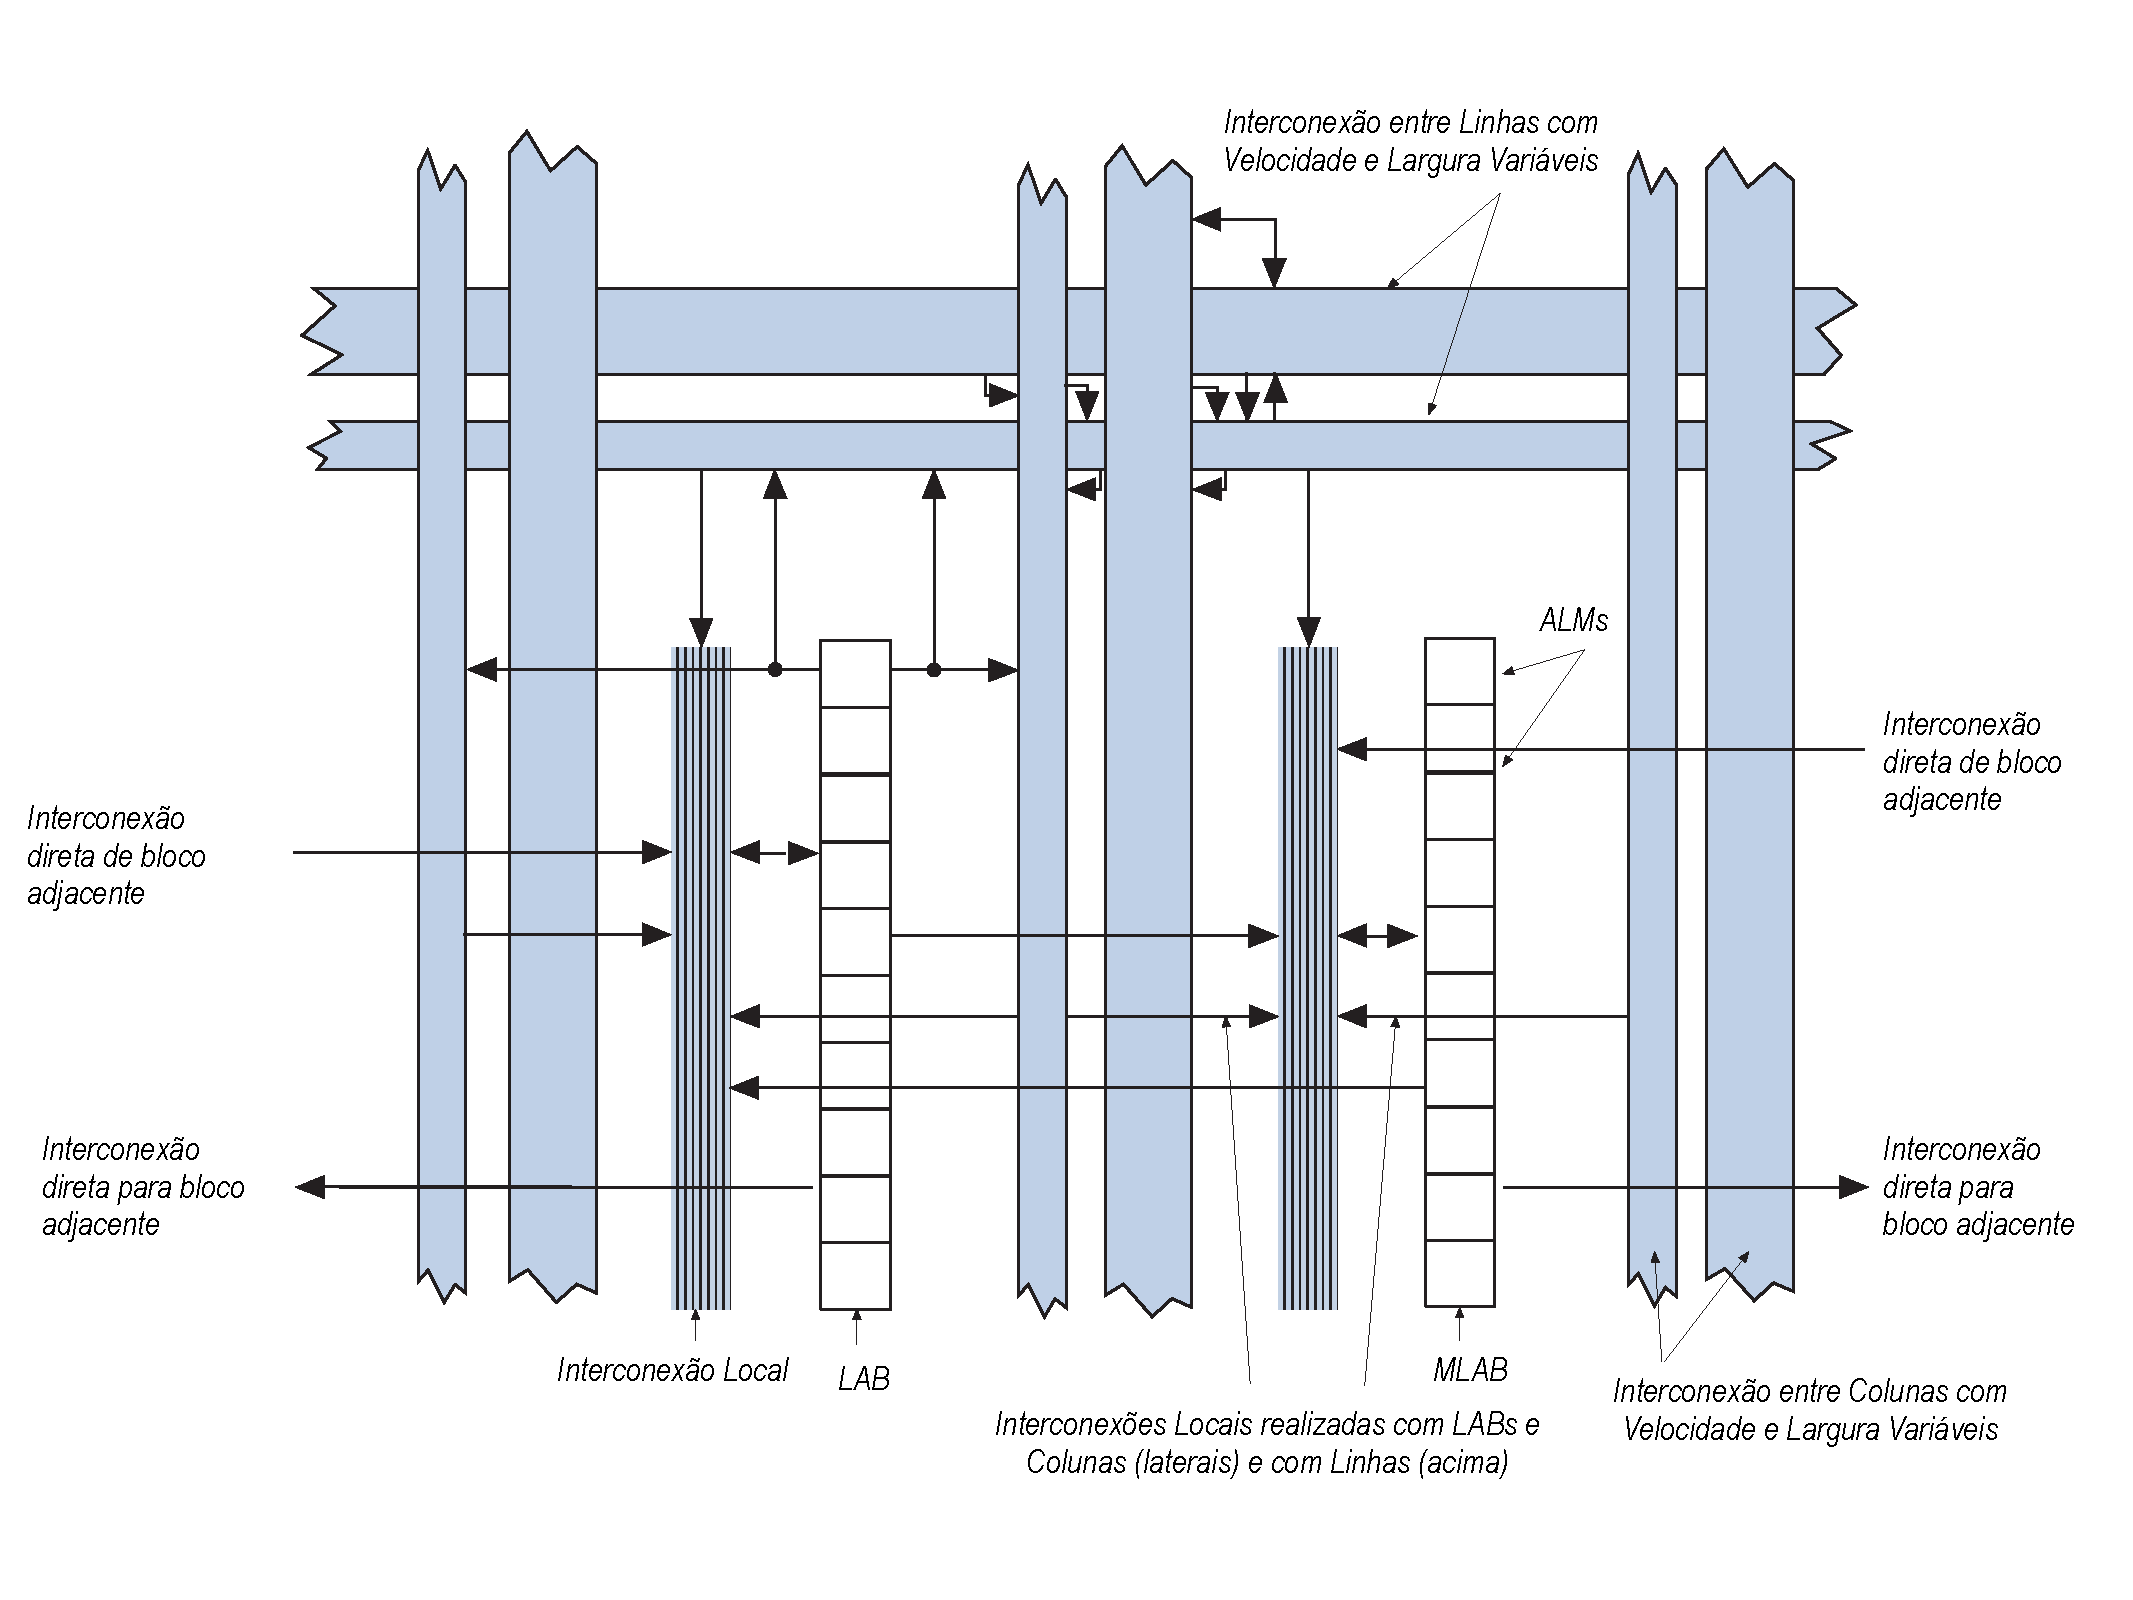
\includegraphics[height=.75\textheight]{stratix_lab}
\end{frame}

\begin{frame}{Altera® Stratix}
	\center	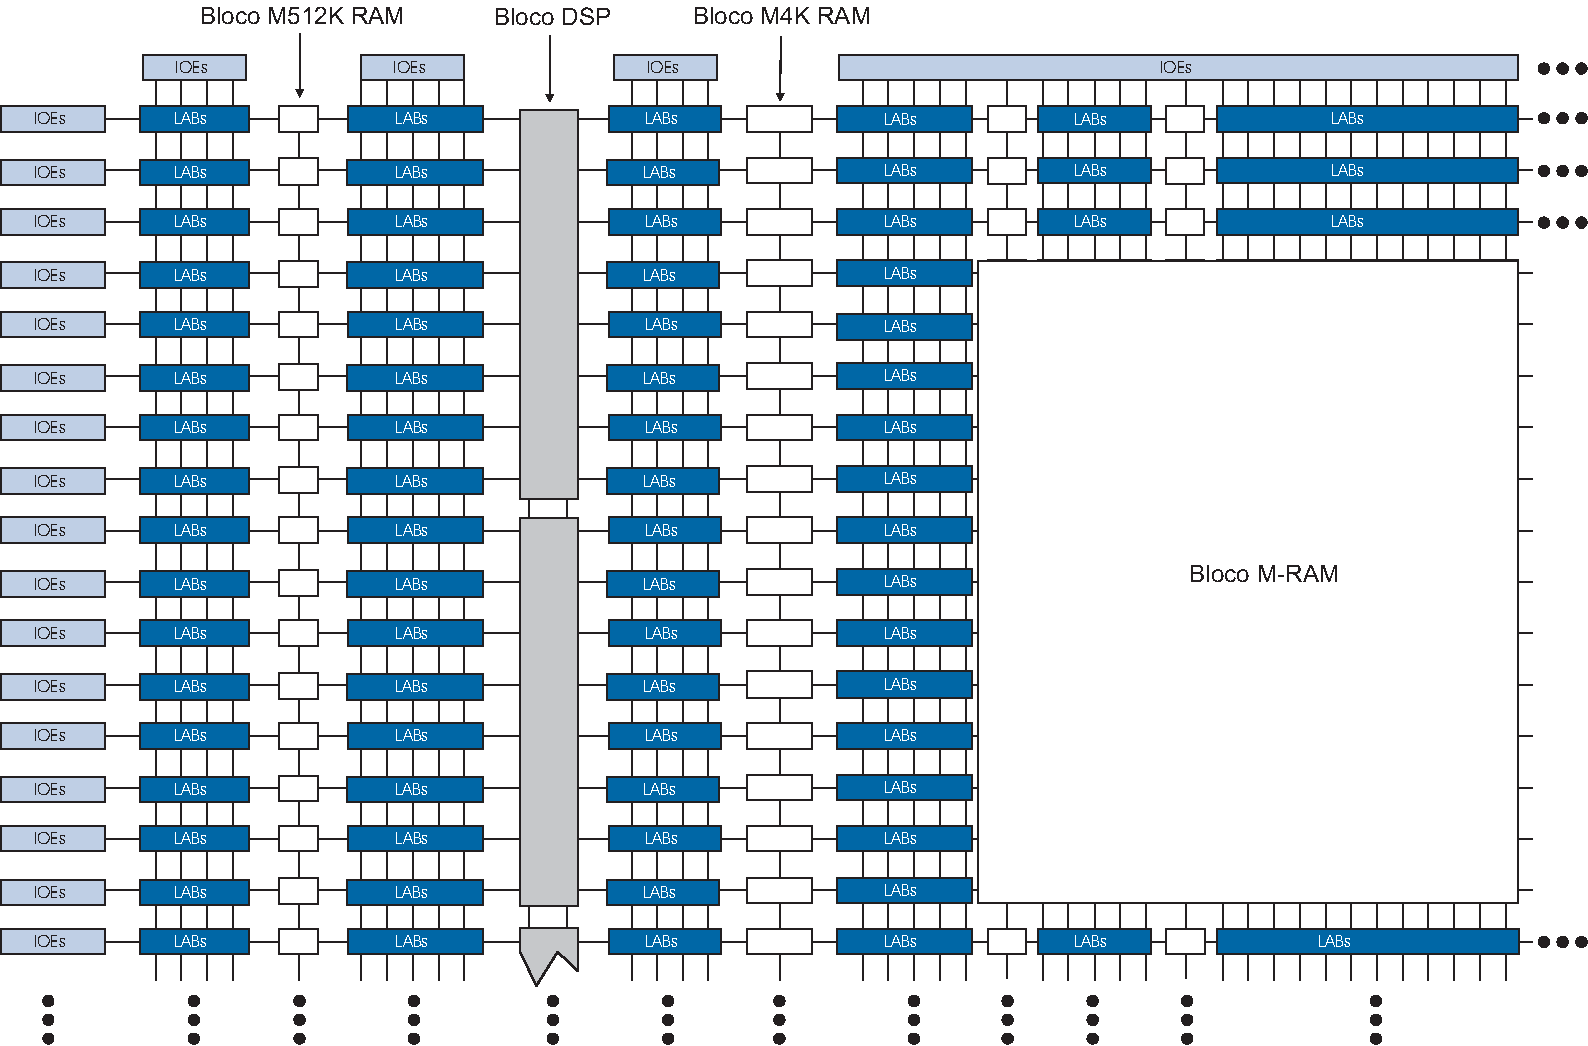
\includegraphics[height=.75\textheight]{stratix}
\end{frame}

\begin{frame}{Fluxo de desenvolvimento para FPGAs \cite{menotti2010.phd}} 
	\center	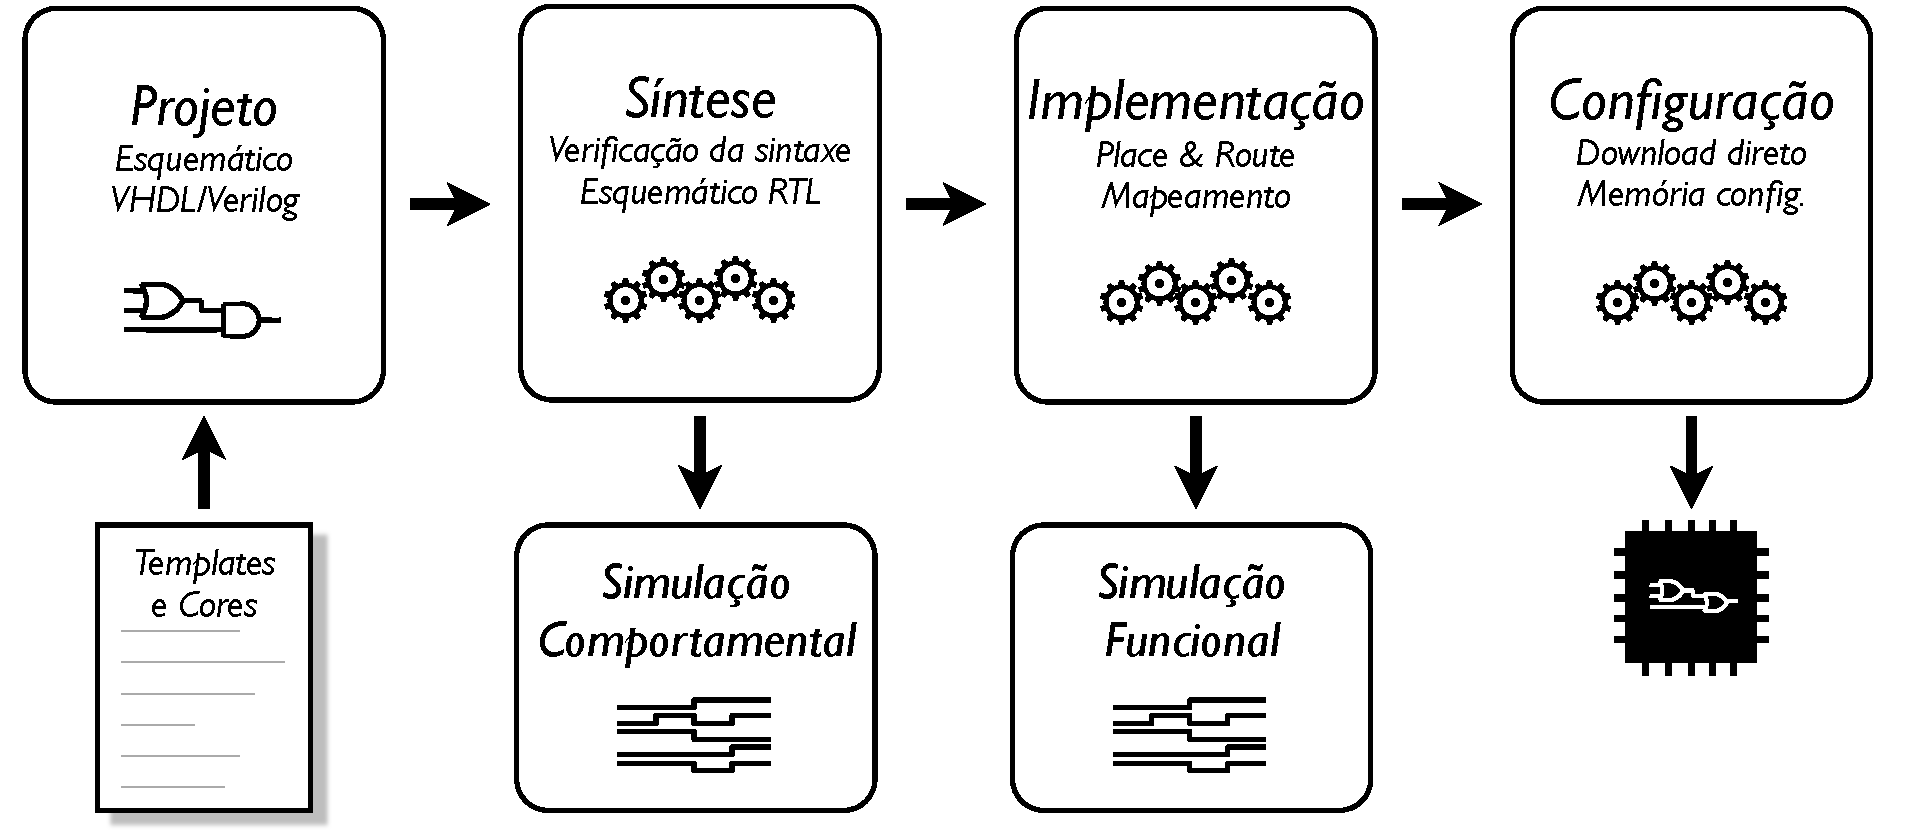
\includegraphics[width=\textwidth]{fpgaflow}
\end{frame}

\begin{frame}{Codesign \cite{micheli}}
	\center	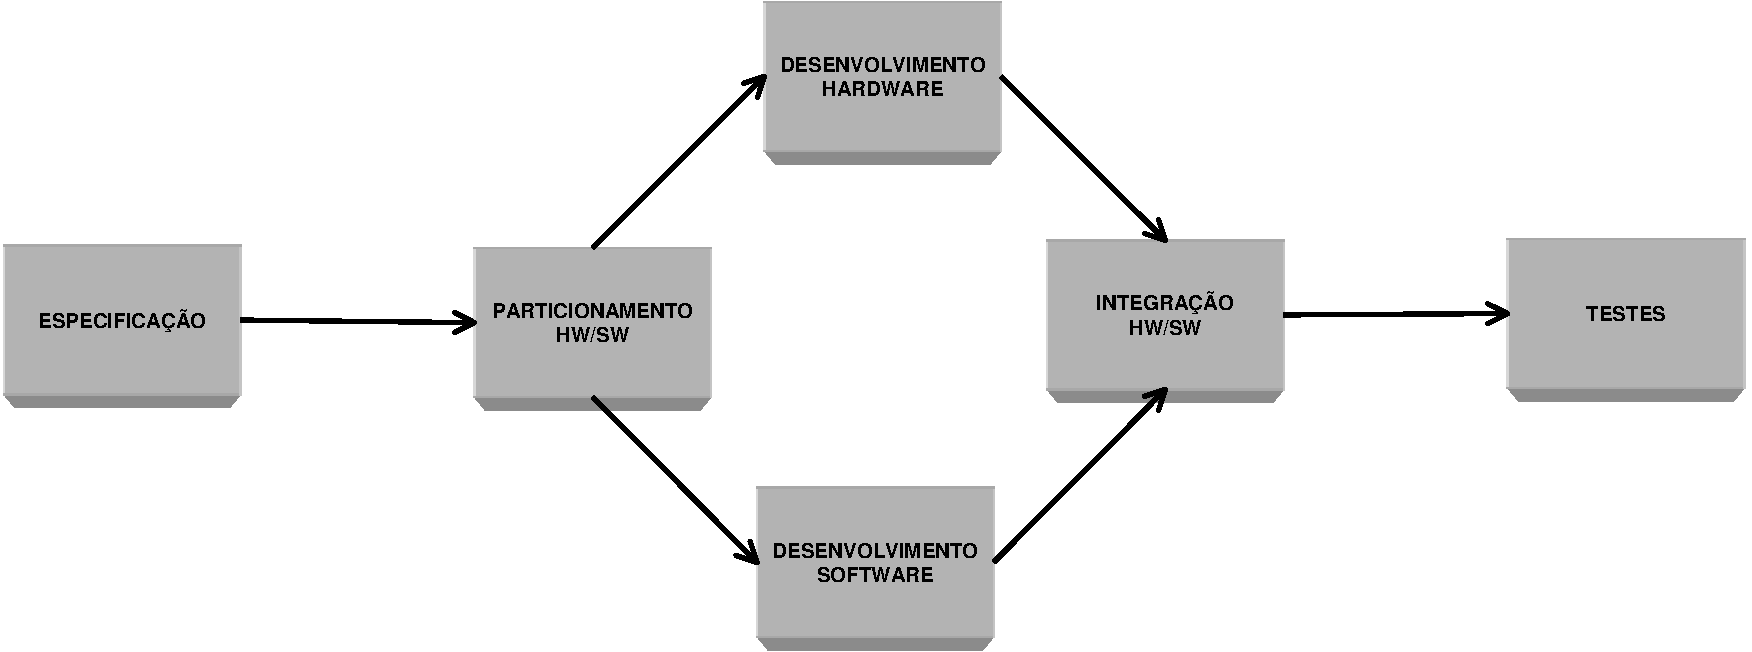
\includegraphics[width=\textwidth]{codesign}
\end{frame}

\section{Aplicações} %%%%%%%%%%%%%%%%%%%%%%%%%%%%%%%%%%%%%%%%%%%%%%%%%%%%%%%%%%%%%%%%%%%%%%

\begin{frame}{\insertsection: Password Crack}{}
\begin{figure}
    \includegraphics<1>[width=.75\textwidth]{Pico_WPA_final_500}
    \includegraphics<2>[width=.75\textwidth]{6M501_}
\end{figure}
\end{frame}

\begin{frame}{\insertsection: Catapult -- Bing -- Microsoft}{\cite{putnam2014}}
	\center	\includegraphics[trim=320 570 50 73, clip, page=2, height=.75\textheight]{Catapult_ISCA_2014}
\end{frame}

\section{Mercado} %%%%%%%%%%%%%%%%%%%%%%%%%%%%%%%%%%%%%%%%%%%%%%%%%%%%%%%%%%%%%%%%%%%%%%

\begin{frame}{\insertsection: CERN}
	\center	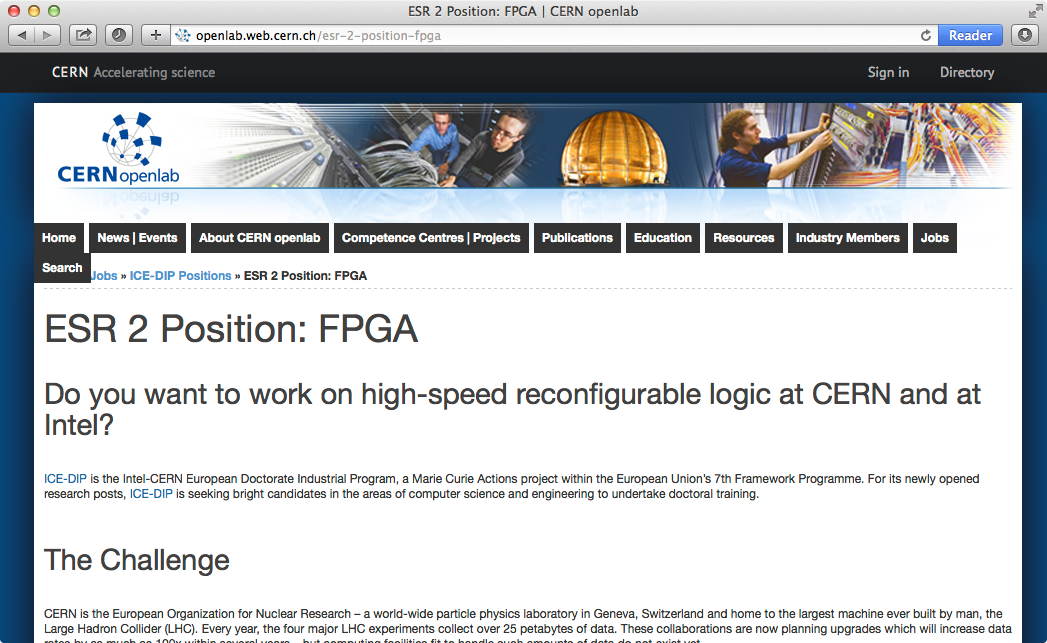
\includegraphics[height=.75\textheight]{PositionCERN}
\end{frame}


\begin{frame}{\insertsection: LNLS} 
	\center	\includegraphics[trim=55 275 55 70, clip, height=.75\textheight]{LNLS_estagio_DIG}
\end{frame}

\begin{frame}[fragile]{\insertsection: CI Brasil}
        \small
	\begin{easylist}[itemize]
        & Programas de Formação        && EDA - Cadence Design System Inc.        & Bolsa
        && R\$ 2.000,00        & Bibliografia Recomendada:        && CMOS VLSI Design: A Circuits and Systems Perspective Neil Weste, David Harris        && Digital Integrated Circuits: A Design Perspective, Jan M. Rabaey, Anantha Chandrakasan, Borivoje Nikolic        && Microeletrônica, Adel S. Sedra, Kenneth C. Smith        && Computer Organization and Design: The Hardware/Software Interface, David A. Patterson, John L. Hennessy	\end{easylist}
\end{frame}

\section{Referências Bibliográficas} %%%%%%%%%%%%%%%%%%%%%%%%%%%%%%%%%%%%%%%%%%%%%%%%%%%%

\begin{frame}[allowframebreaks]{Referências Bibliográficas}
\bibliographystyle{plainnat}
%\bibliographystyle{ieeetr}
\bibliography{refs}
\end{frame}

\end{document}